\documentclass[twoside]{book}

% Packages required by doxygen
\usepackage{calc}
\usepackage{doxygen}
\usepackage{graphicx}
\usepackage[utf8]{inputenc}
\usepackage{makeidx}
\usepackage{multicol}
\usepackage{multirow}
\usepackage{textcomp}
\usepackage[table]{xcolor}

% Font selection
\usepackage[T1]{fontenc}
\usepackage{mathptmx}
\usepackage[scaled=.90]{helvet}
\usepackage{courier}
\usepackage{amssymb}
\usepackage{sectsty}
\renewcommand{\familydefault}{\sfdefault}
\allsectionsfont{%
  \fontseries{bc}\selectfont%
  \color{darkgray}%
}
\renewcommand{\DoxyLabelFont}{%
  \fontseries{bc}\selectfont%
  \color{darkgray}%
}

% Page & text layout
\usepackage{geometry}
\geometry{%
  a4paper,%
  top=2.5cm,%
  bottom=2.5cm,%
  left=2.5cm,%
  right=2.5cm%
}
\tolerance=750
\hfuzz=15pt
\hbadness=750
\setlength{\emergencystretch}{15pt}
\setlength{\parindent}{0cm}
\setlength{\parskip}{0.2cm}
\makeatletter
\renewcommand{\paragraph}{%
  \@startsection{paragraph}{4}{0ex}{-1.0ex}{1.0ex}{%
    \normalfont\normalsize\bfseries\SS@parafont%
  }%
}
\renewcommand{\subparagraph}{%
  \@startsection{subparagraph}{5}{0ex}{-1.0ex}{1.0ex}{%
    \normalfont\normalsize\bfseries\SS@subparafont%
  }%
}
\makeatother

% Headers & footers
\usepackage{fancyhdr}
\pagestyle{fancyplain}
\fancyhead[LE]{\fancyplain{}{\bfseries\thepage}}
\fancyhead[CE]{\fancyplain{}{}}
\fancyhead[RE]{\fancyplain{}{\bfseries\leftmark}}
\fancyhead[LO]{\fancyplain{}{\bfseries\rightmark}}
\fancyhead[CO]{\fancyplain{}{}}
\fancyhead[RO]{\fancyplain{}{\bfseries\thepage}}
\fancyfoot[LE]{\fancyplain{}{}}
\fancyfoot[CE]{\fancyplain{}{}}
\fancyfoot[RE]{\fancyplain{}{\bfseries\scriptsize Generated on Fri Dec 6 2013 21\-:00\-:04 for Student\-Scheduler by Doxygen }}
\fancyfoot[LO]{\fancyplain{}{\bfseries\scriptsize Generated on Fri Dec 6 2013 21\-:00\-:04 for Student\-Scheduler by Doxygen }}
\fancyfoot[CO]{\fancyplain{}{}}
\fancyfoot[RO]{\fancyplain{}{}}
\renewcommand{\footrulewidth}{0.4pt}
\renewcommand{\chaptermark}[1]{%
  \markboth{#1}{}%
}
\renewcommand{\sectionmark}[1]{%
  \markright{\thesection\ #1}%
}

% Indices & bibliography
\usepackage{natbib}
\usepackage[titles]{tocloft}
\setcounter{tocdepth}{3}
\setcounter{secnumdepth}{5}
\makeindex

% Hyperlinks (required, but should be loaded last)
\usepackage{ifpdf}
\ifpdf
  \usepackage[pdftex,pagebackref=true]{hyperref}
\else
  \usepackage[ps2pdf,pagebackref=true]{hyperref}
\fi
\hypersetup{%
  colorlinks=true,%
  linkcolor=blue,%
  citecolor=blue,%
  unicode%
}

% Custom commands
\newcommand{\clearemptydoublepage}{%
  \newpage{\pagestyle{empty}\cleardoublepage}%
}


%===== C O N T E N T S =====

\begin{document}

% Titlepage & ToC
\hypersetup{pageanchor=false}
\pagenumbering{roman}
\begin{titlepage}
\vspace*{7cm}
\begin{center}%
{\Large Student\-Scheduler }\\
\vspace*{1cm}
{\large Generated by Doxygen 1.8.5}\\
\vspace*{0.5cm}
{\small Fri Dec 6 2013 21:00:04}\\
\end{center}
\end{titlepage}
\clearemptydoublepage
\tableofcontents
\clearemptydoublepage
\pagenumbering{arabic}
\hypersetup{pageanchor=true}

%--- Begin generated contents ---
\chapter{Hierarchical Index}
\section{Class Hierarchy}
This inheritance list is sorted roughly, but not completely, alphabetically\-:\begin{DoxyCompactList}
\item Q\-Dialog\begin{DoxyCompactList}
\item \contentsline{section}{Confirmation}{\pageref{class_confirmation}}{}
\item \contentsline{section}{Event}{\pageref{class_event}}{}
\item \contentsline{section}{Main\-Window}{\pageref{class_main_window}}{}
\item \contentsline{section}{Main\-Window}{\pageref{class_main_window}}{}
\item \contentsline{section}{Main\-Window}{\pageref{class_main_window}}{}
\item \contentsline{section}{Main\-Window}{\pageref{class_main_window}}{}
\item \contentsline{section}{Main\-Window}{\pageref{class_main_window}}{}
\item \contentsline{section}{Welcome\-Page}{\pageref{class_welcome_page}}{}
\end{DoxyCompactList}
\item Q\-Main\-Window\begin{DoxyCompactList}
\item \contentsline{section}{Home}{\pageref{class_home}}{}
\end{DoxyCompactList}
\item Q\-Object\begin{DoxyCompactList}
\item \contentsline{section}{My\-Network}{\pageref{class_my_network}}{}
\end{DoxyCompactList}
\item Q\-Tab\-Widget\begin{DoxyCompactList}
\item \contentsline{section}{Scheduler}{\pageref{class_scheduler}}{}
\end{DoxyCompactList}
\end{DoxyCompactList}

\chapter{Class Index}
\section{Class List}
Here are the classes, structs, unions and interfaces with brief descriptions\-:\begin{DoxyCompactList}
\item\contentsline{section}{\hyperlink{class_confirmation}{Confirmation} }{\pageref{class_confirmation}}{}
\item\contentsline{section}{\hyperlink{class_event}{Event} }{\pageref{class_event}}{}
\item\contentsline{section}{\hyperlink{class_home}{Home} }{\pageref{class_home}}{}
\item\contentsline{section}{\hyperlink{class_main_window}{Main\-Window} }{\pageref{class_main_window}}{}
\item\contentsline{section}{\hyperlink{class_my_network}{My\-Network} }{\pageref{class_my_network}}{}
\item\contentsline{section}{\hyperlink{class_scheduler}{Scheduler} }{\pageref{class_scheduler}}{}
\item\contentsline{section}{\hyperlink{class_welcome_page}{Welcome\-Page} }{\pageref{class_welcome_page}}{}
\end{DoxyCompactList}

\chapter{Class Documentation}
\hypertarget{class_confirmation}{\section{Confirmation Class Reference}
\label{class_confirmation}\index{Confirmation@{Confirmation}}
}
Inheritance diagram for Confirmation\-:\begin{figure}[H]
\begin{center}
\leavevmode
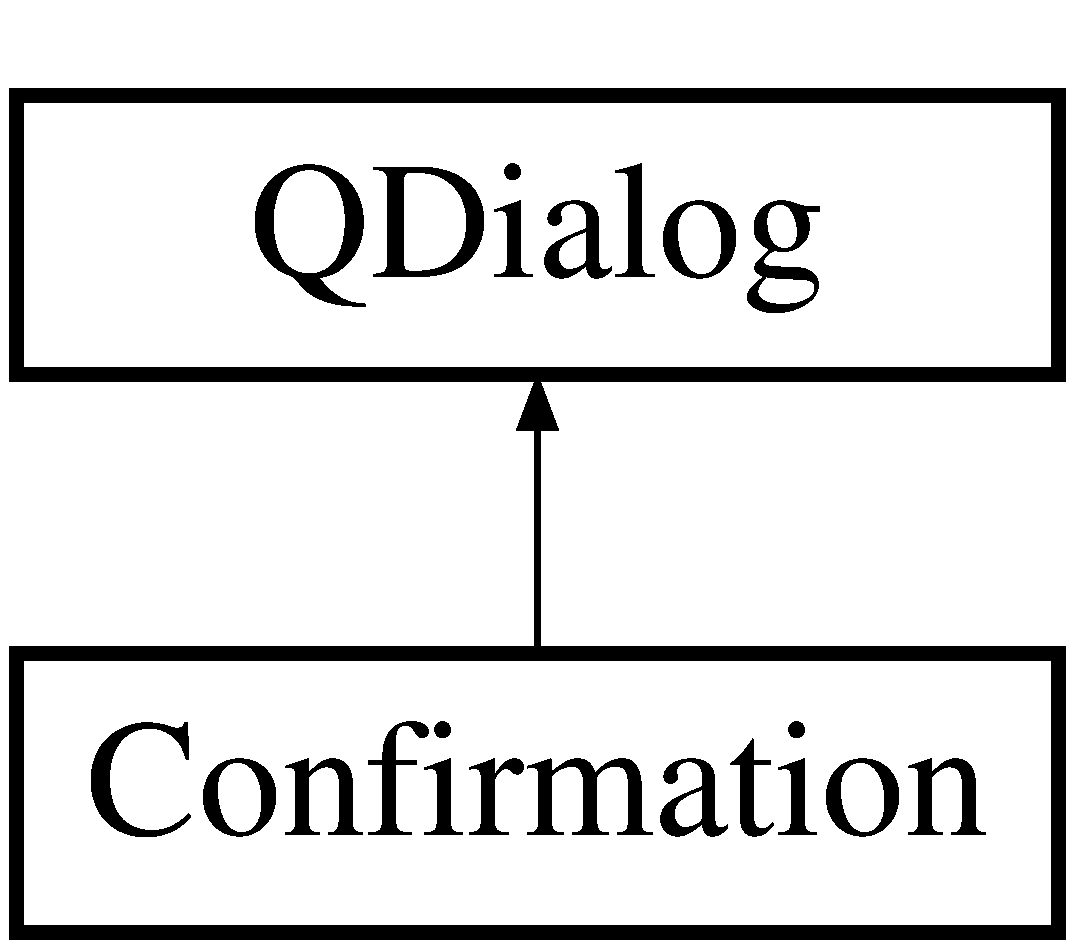
\includegraphics[height=2.000000cm]{class_confirmation}
\end{center}
\end{figure}
\subsection*{Public Member Functions}
\begin{DoxyCompactItemize}
\item 
\hypertarget{class_confirmation_a96bd3ae5935e5b5f00de22ff102d6458}{{\bfseries Confirmation} (Q\-Widget $\ast$parent=0)}\label{class_confirmation_a96bd3ae5935e5b5f00de22ff102d6458}

\item 
\hypertarget{class_confirmation_ab15191d758e5993be6ccf0ea751e00f6}{void {\bfseries created\-Account} ()}\label{class_confirmation_ab15191d758e5993be6ccf0ea751e00f6}

\item 
\hypertarget{class_confirmation_adec23882d8de468c7a27bec428ebd75e}{void {\bfseries created\-Semester} ()}\label{class_confirmation_adec23882d8de468c7a27bec428ebd75e}

\item 
\hypertarget{class_confirmation_a27774940db2a184a38cd931dd0e3af73}{void {\bfseries created\-Holiday} ()}\label{class_confirmation_a27774940db2a184a38cd931dd0e3af73}

\item 
\hypertarget{class_confirmation_aec0592bb428c30abf2b4b5dea7ebfc39}{void {\bfseries created\-Class} ()}\label{class_confirmation_aec0592bb428c30abf2b4b5dea7ebfc39}

\item 
\hypertarget{class_confirmation_af5ae70cdf537de5cb58f0caad4048c20}{void {\bfseries created\-Event} ()}\label{class_confirmation_af5ae70cdf537de5cb58f0caad4048c20}

\end{DoxyCompactItemize}


The documentation for this class was generated from the following files\-:\begin{DoxyCompactItemize}
\item 
/\-Users/macanrox/studentscheduler/confirmation.\-h\item 
/\-Users/macanrox/studentscheduler/confirmation.\-cpp\end{DoxyCompactItemize}

\hypertarget{class_event}{\section{Event Class Reference}
\label{class_event}\index{Event@{Event}}
}
Inheritance diagram for Event\-:\begin{figure}[H]
\begin{center}
\leavevmode
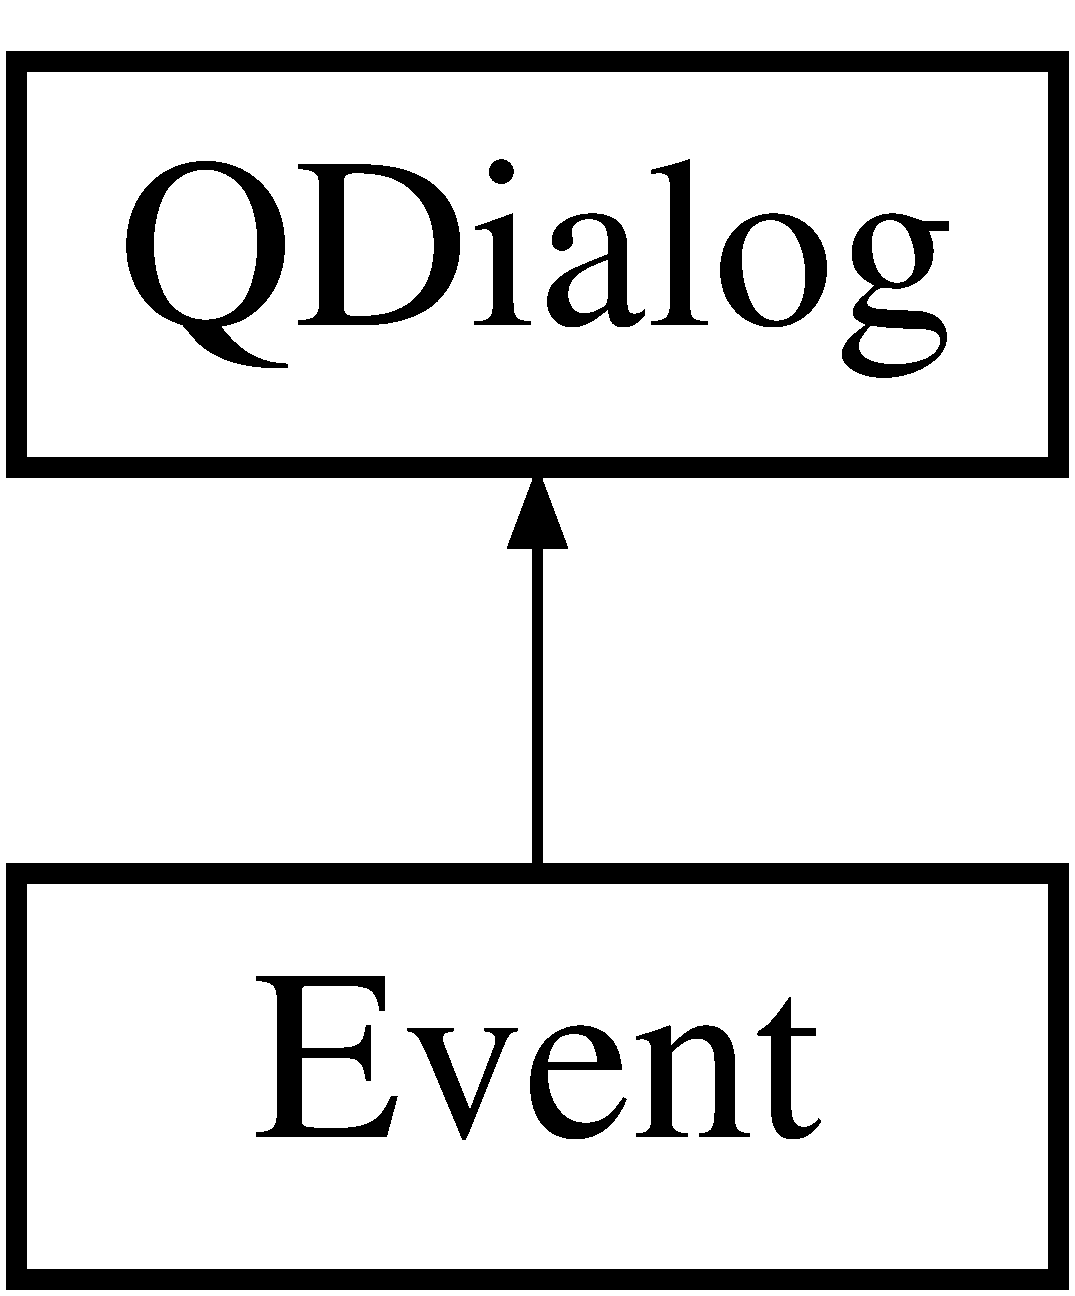
\includegraphics[height=2.000000cm]{class_event}
\end{center}
\end{figure}
\subsection*{Public Member Functions}
\begin{DoxyCompactItemize}
\item 
\hypertarget{class_event_a02c9634eb9174410221f9459a54d7b7f}{{\bfseries Event} (Q\-Widget $\ast$parent=0)}\label{class_event_a02c9634eb9174410221f9459a54d7b7f}

\item 
\hypertarget{class_event_afd2884ff536f352fb4e18debf464f054}{void {\bfseries set\-Class\-I\-D} (Q\-String u)}\label{class_event_afd2884ff536f352fb4e18debf464f054}

\item 
\hypertarget{class_event_a5ab5b77b1671c8346fe8233eecd4f097}{void {\bfseries set\-User\-I\-D} (Q\-String u)}\label{class_event_a5ab5b77b1671c8346fe8233eecd4f097}

\end{DoxyCompactItemize}
\subsection*{Public Attributes}
\begin{DoxyCompactItemize}
\item 
\hypertarget{class_event_a8c3804a90d58066d02c51a0cc6890bac}{Q\-String {\bfseries class\-I\-D}}\label{class_event_a8c3804a90d58066d02c51a0cc6890bac}

\item 
\hypertarget{class_event_a9b3528e0db0f3a842ca9b4be33743ca8}{Q\-String {\bfseries user\-I\-D}}\label{class_event_a9b3528e0db0f3a842ca9b4be33743ca8}

\end{DoxyCompactItemize}


The documentation for this class was generated from the following files\-:\begin{DoxyCompactItemize}
\item 
/\-Users/macanrox/studentscheduler/event.\-h\item 
/\-Users/macanrox/studentscheduler/event.\-cpp\end{DoxyCompactItemize}

\hypertarget{class_home}{\section{Home Class Reference}
\label{class_home}\index{Home@{Home}}
}
Inheritance diagram for Home\-:\begin{figure}[H]
\begin{center}
\leavevmode
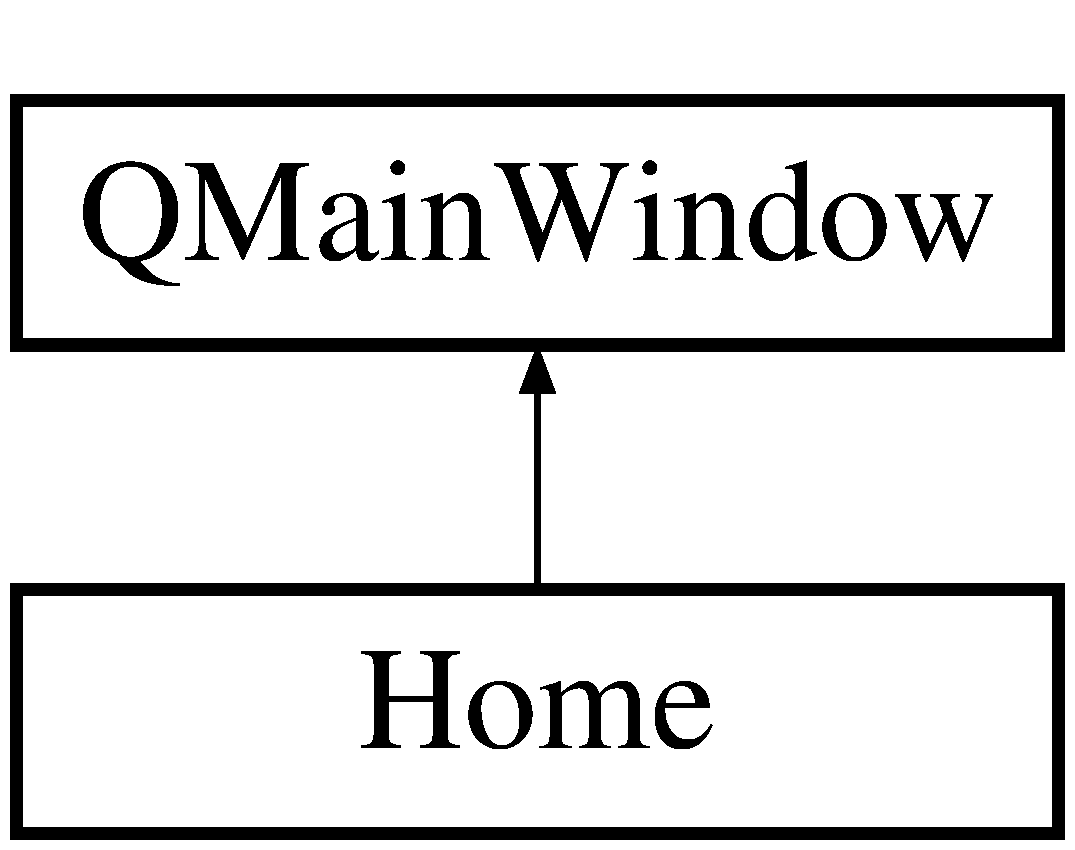
\includegraphics[height=2.000000cm]{class_home}
\end{center}
\end{figure}
\subsection*{Public Member Functions}
\begin{DoxyCompactItemize}
\item 
\hypertarget{class_home_aeedf0ef0f57ed0b071106f3db10813df}{{\bfseries Home} (Q\-Widget $\ast$parent=0)}\label{class_home_aeedf0ef0f57ed0b071106f3db10813df}

\end{DoxyCompactItemize}


The documentation for this class was generated from the following files\-:\begin{DoxyCompactItemize}
\item 
/\-Users/macanrox/studentscheduler/home.\-h\item 
/\-Users/macanrox/studentscheduler/home.\-cpp\end{DoxyCompactItemize}

\hypertarget{class_main_window}{\section{Main\-Window Class Reference}
\label{class_main_window}\index{Main\-Window@{Main\-Window}}
}
Inheritance diagram for Main\-Window\-:\begin{figure}[H]
\begin{center}
\leavevmode
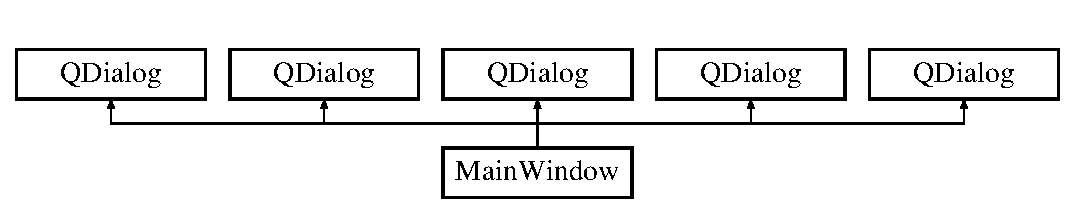
\includegraphics[height=2.000000cm]{class_main_window}
\end{center}
\end{figure}
\subsection*{Public Member Functions}
\begin{DoxyCompactItemize}
\item 
\hypertarget{class_main_window_a8b244be8b7b7db1b08de2a2acb9409db}{{\bfseries Main\-Window} (Q\-Widget $\ast$parent=0)}\label{class_main_window_a8b244be8b7b7db1b08de2a2acb9409db}

\item 
\hypertarget{class_main_window_a05931820affb5e30b4dcc46bdf32e75e}{void {\bfseries set\-Hi\-User\-Text} ()}\label{class_main_window_a05931820affb5e30b4dcc46bdf32e75e}

\item 
\hypertarget{class_main_window_a348aac0acc219ec317294308f6fa618b}{void {\bfseries set\-User\-I\-D} (Q\-String u)}\label{class_main_window_a348aac0acc219ec317294308f6fa618b}

\item 
\hypertarget{class_main_window_a2436f8c6685172068604c43c25709040}{void {\bfseries set\-Global\-Object} (Q\-Byte\-Array u)}\label{class_main_window_a2436f8c6685172068604c43c25709040}

\item 
\hypertarget{class_main_window_a1ac1c3e1eb71f7b08800559898e7bac5}{void {\bfseries confirmation\-Window} (int i)}\label{class_main_window_a1ac1c3e1eb71f7b08800559898e7bac5}

\item 
\hypertarget{class_main_window_a8b244be8b7b7db1b08de2a2acb9409db}{{\bfseries Main\-Window} (Q\-Widget $\ast$parent=0)}\label{class_main_window_a8b244be8b7b7db1b08de2a2acb9409db}

\item 
\hypertarget{class_main_window_ab1d0cc488a9fcaa215e13413e05d20a3}{void {\bfseries set\-Hi\-User\-Text} (Q\-String hi\-Text)}\label{class_main_window_ab1d0cc488a9fcaa215e13413e05d20a3}

\item 
\hypertarget{class_main_window_a8b244be8b7b7db1b08de2a2acb9409db}{{\bfseries Main\-Window} (Q\-Widget $\ast$parent=0)}\label{class_main_window_a8b244be8b7b7db1b08de2a2acb9409db}

\item 
\hypertarget{class_main_window_a8b244be8b7b7db1b08de2a2acb9409db}{{\bfseries Main\-Window} (Q\-Widget $\ast$parent=0)}\label{class_main_window_a8b244be8b7b7db1b08de2a2acb9409db}

\item 
\hypertarget{class_main_window_ab1d0cc488a9fcaa215e13413e05d20a3}{void {\bfseries set\-Hi\-User\-Text} (Q\-String hi\-Text)}\label{class_main_window_ab1d0cc488a9fcaa215e13413e05d20a3}

\item 
\hypertarget{class_main_window_a8b244be8b7b7db1b08de2a2acb9409db}{{\bfseries Main\-Window} (Q\-Widget $\ast$parent=0)}\label{class_main_window_a8b244be8b7b7db1b08de2a2acb9409db}

\item 
\hypertarget{class_main_window_ab1d0cc488a9fcaa215e13413e05d20a3}{void {\bfseries set\-Hi\-User\-Text} (Q\-String hi\-Text)}\label{class_main_window_ab1d0cc488a9fcaa215e13413e05d20a3}

\item 
\hypertarget{class_main_window_a348aac0acc219ec317294308f6fa618b}{void {\bfseries set\-User\-I\-D} (Q\-String u)}\label{class_main_window_a348aac0acc219ec317294308f6fa618b}

\end{DoxyCompactItemize}
\subsection*{Public Attributes}
\begin{DoxyCompactItemize}
\item 
\hypertarget{class_main_window_a9f66bfa4a75719a5045fbd4f1af616cf}{Q\-Byte\-Array {\bfseries global\-Objects}}\label{class_main_window_a9f66bfa4a75719a5045fbd4f1af616cf}

\item 
\hypertarget{class_main_window_a47496802a6ea3712bcdbe86aacbfe63e}{Q\-String {\bfseries user\-I\-D}}\label{class_main_window_a47496802a6ea3712bcdbe86aacbfe63e}

\end{DoxyCompactItemize}


The documentation for this class was generated from the following files\-:\begin{DoxyCompactItemize}
\item 
/\-Users/macanrox/studentscheduler/mainwindow.\-h\item 
/\-Users/macanrox/studentscheduler/mainwindow.\-h.\-B\-A\-C\-K\-U\-P.\-12072.\-h\item 
/\-Users/macanrox/studentscheduler/mainwindow.\-h.\-B\-A\-S\-E.\-12072.\-h\item 
/\-Users/macanrox/studentscheduler/mainwindow.\-h.\-L\-O\-C\-A\-L.\-12072.\-h\item 
/\-Users/macanrox/studentscheduler/mainwindow.\-h.\-R\-E\-M\-O\-T\-E.\-12072.\-h\item 
/\-Users/macanrox/studentscheduler/mainwindow.\-cpp\end{DoxyCompactItemize}

\hypertarget{class_my_network}{\section{My\-Network Class Reference}
\label{class_my_network}\index{My\-Network@{My\-Network}}
}
Inheritance diagram for My\-Network\-:\begin{figure}[H]
\begin{center}
\leavevmode
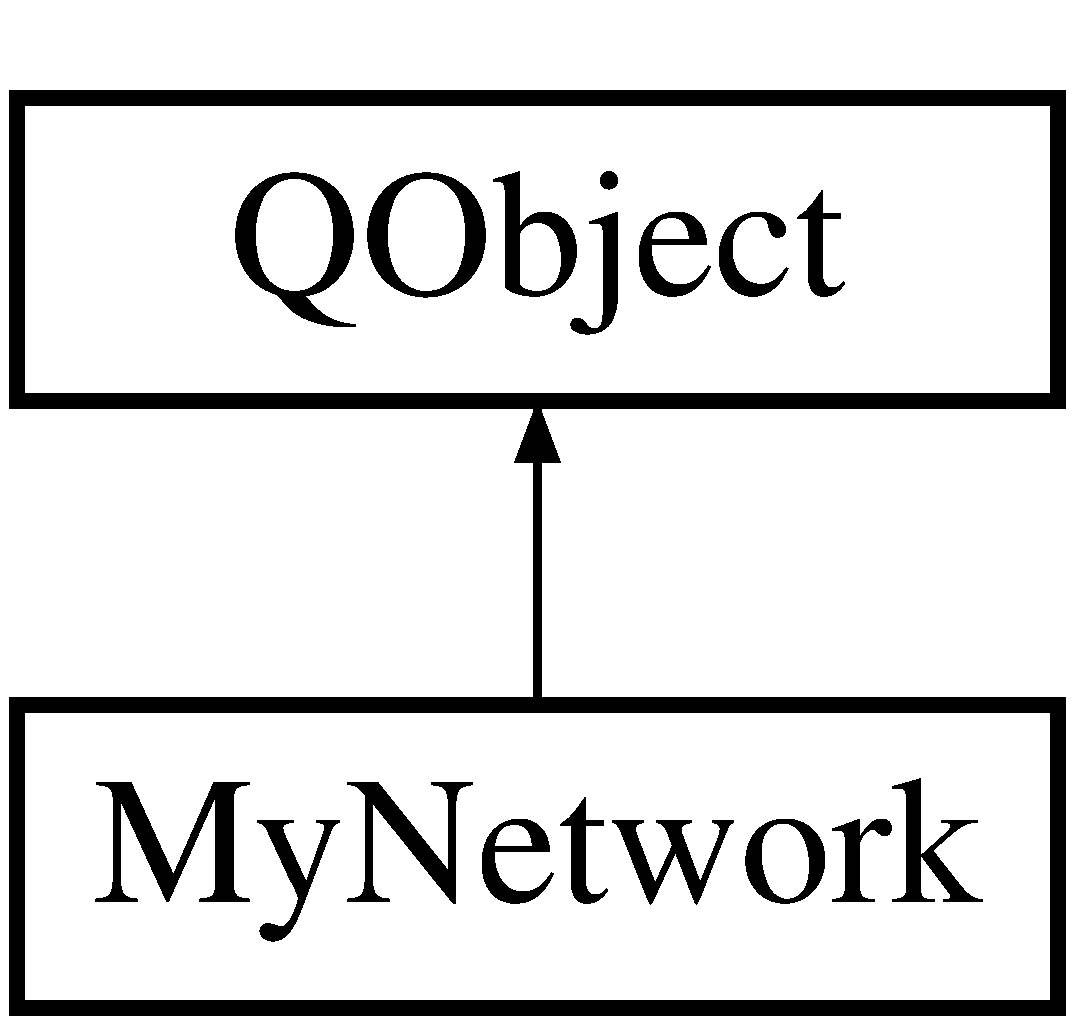
\includegraphics[height=2.000000cm]{class_my_network}
\end{center}
\end{figure}
\subsection*{Public Slots}
\begin{DoxyCompactItemize}
\item 
\hypertarget{class_my_network_af59760d3b07e8fb4d04ee12b0f10c62d}{void {\bfseries set\-Response} (Q\-Network\-Reply $\ast$reply)}\label{class_my_network_af59760d3b07e8fb4d04ee12b0f10c62d}

\end{DoxyCompactItemize}
\subsection*{Signals}
\begin{DoxyCompactItemize}
\item 
\hypertarget{class_my_network_a1e8cdf0cd32c60a2c573aa0016fd8783}{Q\-String {\bfseries done\-Post} (\hyperlink{class_my_network}{My\-Network} $\ast$my\-Post)}\label{class_my_network_a1e8cdf0cd32c60a2c573aa0016fd8783}

\end{DoxyCompactItemize}
\subsection*{Public Member Functions}
\begin{DoxyCompactItemize}
\item 
\hypertarget{class_my_network_a2d3f8f7fdd0121033cf6161d1e87981e}{void {\bfseries set\-Post} (const Q\-String \&the\-Key, const Q\-String \&the\-Value)}\label{class_my_network_a2d3f8f7fdd0121033cf6161d1e87981e}

\item 
\hypertarget{class_my_network_a8f2316099203c6ae2cb92075b6e6a671}{void {\bfseries send\-Post} ()}\label{class_my_network_a8f2316099203c6ae2cb92075b6e6a671}

\end{DoxyCompactItemize}
\subsection*{Public Attributes}
\begin{DoxyCompactItemize}
\item 
\hypertarget{class_my_network_afcd1907135594e46dcd19636ce4fe18b}{Q\-Byte\-Array {\bfseries post\-Data}}\label{class_my_network_afcd1907135594e46dcd19636ce4fe18b}

\item 
\hypertarget{class_my_network_a9c038e93302dd30ae02efbfaadec2851}{Q\-Byte\-Array {\bfseries the\-Response}}\label{class_my_network_a9c038e93302dd30ae02efbfaadec2851}

\end{DoxyCompactItemize}


The documentation for this class was generated from the following files\-:\begin{DoxyCompactItemize}
\item 
/\-Users/macanrox/studentscheduler/mynetwork.\-h\item 
/\-Users/macanrox/studentscheduler/mynetwork.\-cpp\end{DoxyCompactItemize}

\hypertarget{class_scheduler}{\section{Scheduler Class Reference}
\label{class_scheduler}\index{Scheduler@{Scheduler}}
}
Inheritance diagram for Scheduler\-:\begin{figure}[H]
\begin{center}
\leavevmode
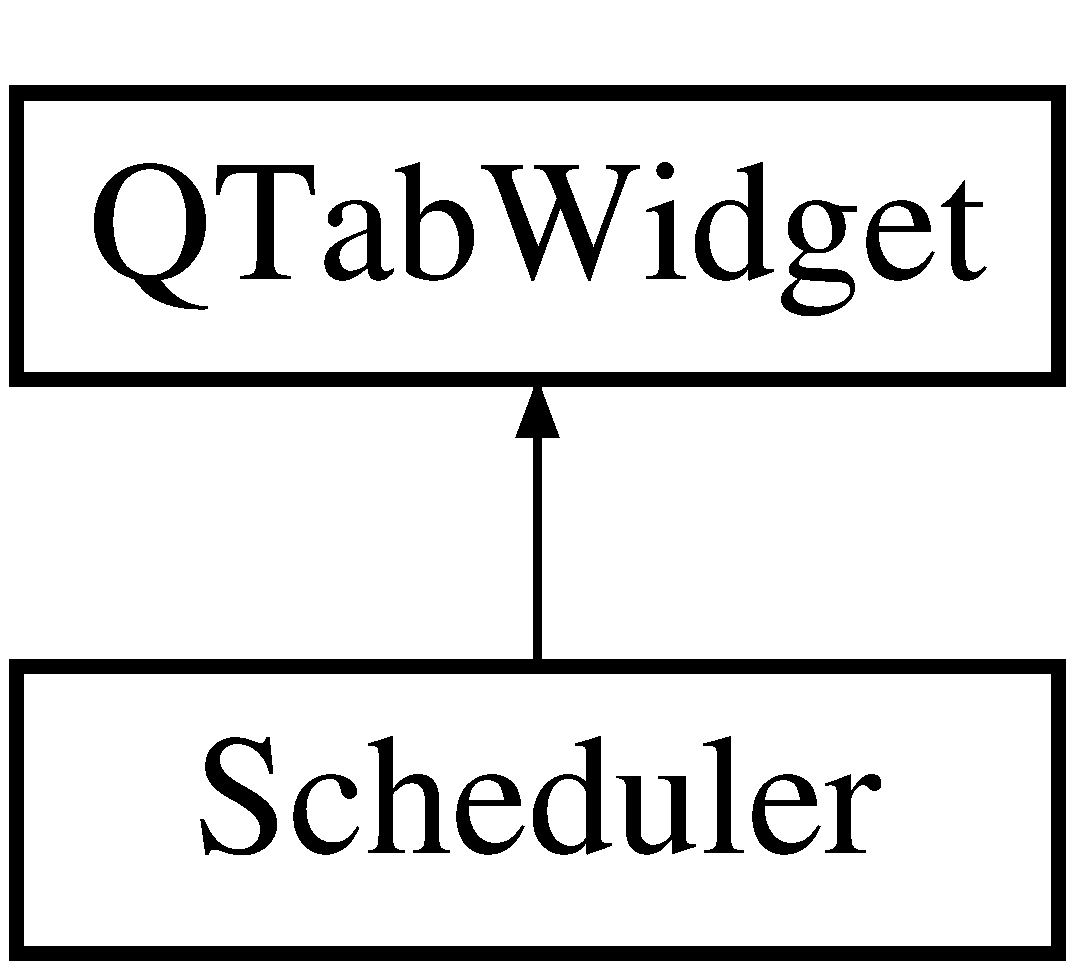
\includegraphics[height=2.000000cm]{class_scheduler}
\end{center}
\end{figure}
\subsection*{Public Member Functions}
\begin{DoxyCompactItemize}
\item 
\hypertarget{class_scheduler_a0343ae3b4e0bfad59da1f45abf2ac5e9}{{\bfseries Scheduler} (Q\-Widget $\ast$parent=0)}\label{class_scheduler_a0343ae3b4e0bfad59da1f45abf2ac5e9}

\end{DoxyCompactItemize}


The documentation for this class was generated from the following files\-:\begin{DoxyCompactItemize}
\item 
/\-Users/macanrox/studentscheduler/scheduler.\-h\item 
/\-Users/macanrox/studentscheduler/scheduler.\-cpp\end{DoxyCompactItemize}

\hypertarget{class_welcome_page}{\section{Welcome\-Page Class Reference}
\label{class_welcome_page}\index{Welcome\-Page@{Welcome\-Page}}
}
Inheritance diagram for Welcome\-Page\-:\begin{figure}[H]
\begin{center}
\leavevmode
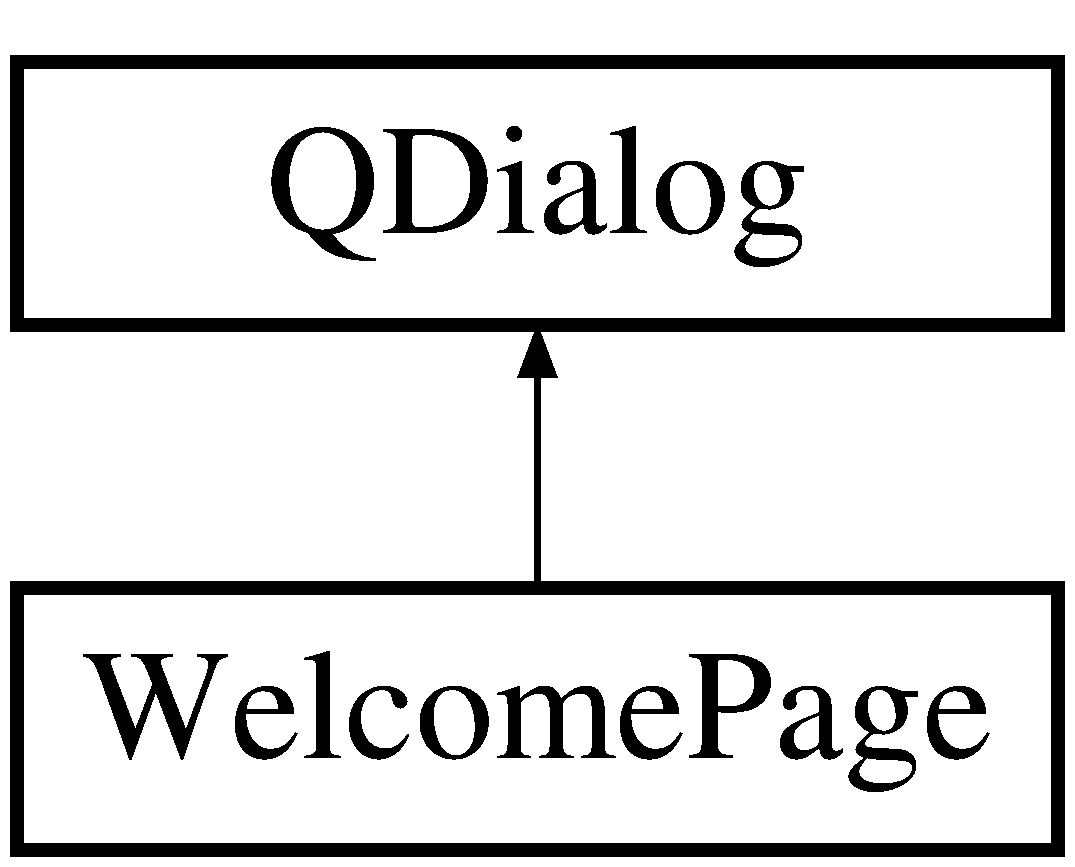
\includegraphics[height=2.000000cm]{class_welcome_page}
\end{center}
\end{figure}
\subsection*{Public Member Functions}
\begin{DoxyCompactItemize}
\item 
\hypertarget{class_welcome_page_a2759d56822391251162b7052772e33b9}{{\bfseries Welcome\-Page} (Q\-Widget $\ast$parent=0)}\label{class_welcome_page_a2759d56822391251162b7052772e33b9}

\end{DoxyCompactItemize}


The documentation for this class was generated from the following files\-:\begin{DoxyCompactItemize}
\item 
/\-Users/macanrox/studentscheduler/welcomepage.\-h\item 
/\-Users/macanrox/studentscheduler/welcomepage.\-cpp\end{DoxyCompactItemize}

%--- End generated contents ---

% Index
\newpage
\phantomsection
\addcontentsline{toc}{part}{Index}
\printindex

\end{document}
